\scanpage{10}
Groupes loc. lib. en car. $p$ (pas néc. annu par $p$)

a) Cristal de prés. finie sur $S_{\mathrm{cris}}/\deleted{\unsure{\mathbb F_p}}\mathbb Z_p$

\deleted{(\unsure{pas néc. lib.} \unsure{De dim pro}}
d'amplitude parfaite $\subset[-1,0]$, soit $\mathcal M$,
avec structures $F_{\mathcal M}$ et $V_{\mathcal M}$.

\deleted{\unsure{b)}}
On en déduit deux triangles exacts de complexes avec $F,V$ sur $S_{\mathrm{cris}}/\mathbb F_p$

$(\mathrm I)$
\diagram{\begin{tikzcd}[column sep=small]
&\mathcal M\overset L\otimes/V\arrow[dl,"\partial_{\mathrm I}"']&\\
\mathcal M\overset L\otimes/F\arrow[rr,"i_{\mathrm I}"]&&\mathcal M^{(p)}\overset L\otimes/p\simeq\varphi^*(\Delta^*)\arrow[ul,"\pi_{\mathrm I}"']
\end{tikzcd}}
\margin{$\Delta^*=\varepsilon^*(\mathbb\Delta^*)$}
\deleted{$\unsure{\mathbb\Delta^*(\mathcal M)}$}

$(\mathrm {II})$
\diagram{\begin{tikzcd}[column sep=small]
&\mathcal M\overset L\otimes/F\arrow[dl]&\\
\mathcal M\overset L\otimes/V\arrow[rr]&&\mathcal M\overset L\otimes/p=\mathbb\Delta^*\arrow[ul]\arrow[d,equal,"\mathrm{dfn}"]\\
&&L\alpha^*(\mathcal M)
\end{tikzcd}}
\margin{$\alpha:S_{\mathrm{cris}}/\mathbb F_p\longrightarrow S_{\mathrm{cris}}/\mathbb Z_p$}

b) \deleted{\unsure{Complexe}} Descente à $S_{\mathrm{zar}}$ (via $\varphi$) de la ``filtration'' $(\mathrm I)$ sur $\varphi^*(\Delta^*)$, en un triangle exact
\diagram{\begin{tikzcd}&\check\ell'_{\bullet}\arrow[dl,"\partial_0"']&\\\ell_{\bullet}[-1]\arrow[rr,"i_0"]&&\Delta^*\arrow[ul,"\pi_0"']\end{tikzcd}}
\figure{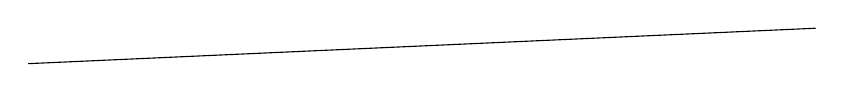
\begin{tikzpicture}\draw(0,0)--(10,.45);\end{tikzpicture}}

Prolongement à un \unsure{épaississement} p. div. $S'$ de $S$
(\unsure{c.à.d.} avec $\unsure{S}=\uline{\operatorname{Var}}(p.1_S)$) On considère
\[
\mathcal M\overset L\otimes\mathcal O_{S'}=\Delta^*(S'),
\]
qui prolonge $\Delta^*$, et il faut se donner un prolongement de la filtration b) de $\Delta^*$ en
\diagram{\begin{tikzcd}&\overline{\check\ell'_{\bullet}}\arrow[dl,"\bar\partial_0"']&\\\bar\ell_{\bullet}[-1]\arrow[rr,dash,"\bar i_0"]&&\Delta^*(S')\arrow[ul,"\pi_0"']\end{tikzcd}}
\mspage{9}
